\section{Introduction}
\label{sec:introduction}

Reconstruction of neuronal morphology is of great significance for brain studies. Obtaining a blue print of the brain architecture, including the morphologies and interconnectivities of neuronal populations, allows for measuring and visualizing neuronal structure, understanding neuronal identity, and determining potential connectivity.
Therefore, complete reconstruction of neuronal populations from large-scale brain images is essential to investigate the mechanism of the nervous system, analyze brain changes, and facilitate our understanding of how the brain works or fails to work properly in the diseases such as dementia and Alzheimer's disease~\cite{Petrella2003, Giorgio2013}.
One of the key techniques in this endeavor is optical microscopy (OM), which allows detailed visualization of neurons and makes the reconstruction of every neuron possible~\cite{Senft2011}, as shown in Fig.~\ref{fig:brain}.
However, despite numerous efforts devoted, this task is still one of the main challenges in computational neuroscience.

\begin{figure}[t]
	\centering
	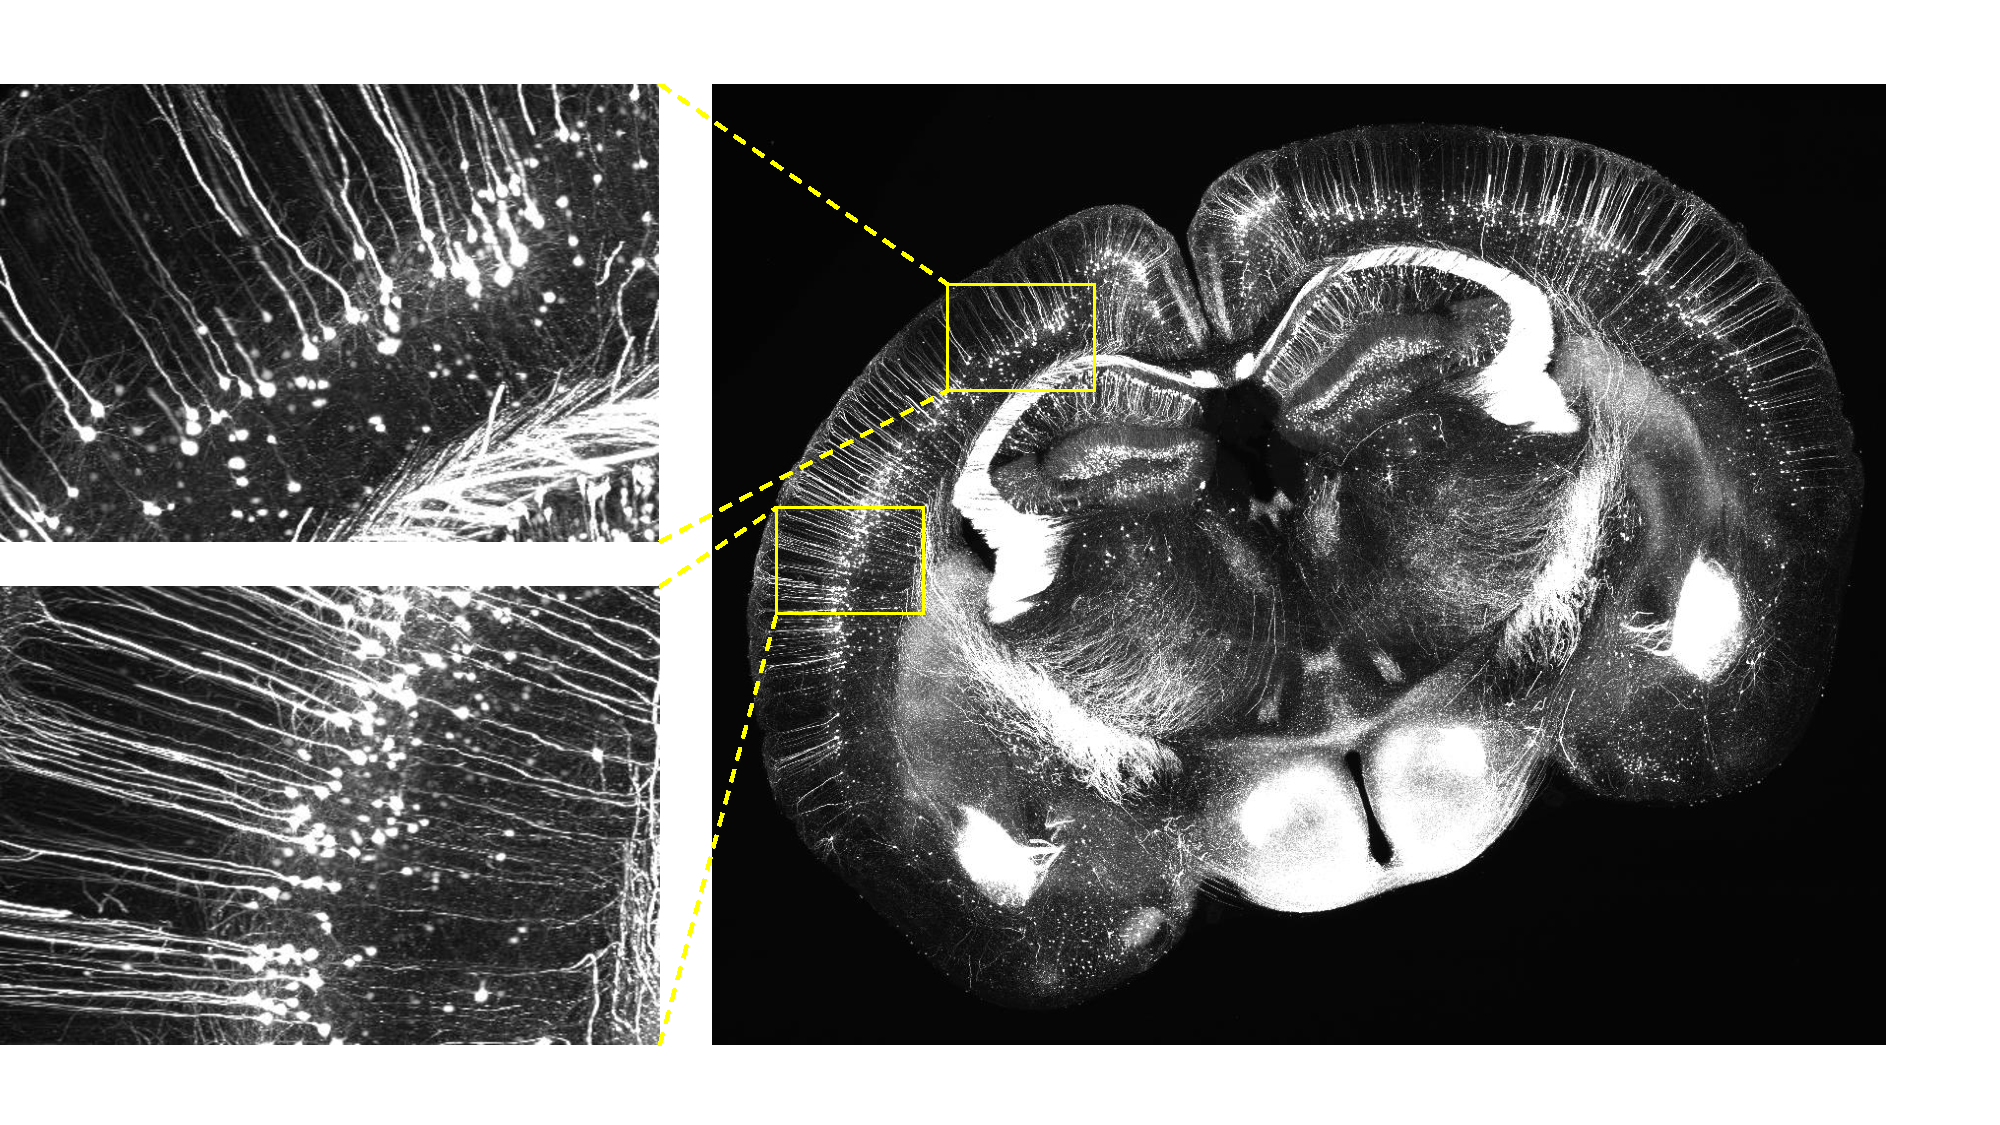
\includegraphics[width=1\columnwidth]{./Illustrations/brain2.pdf}
	\caption{A 3D mouse brain slice captured by the VISoR imaging system~\cite{Wang2019}. The dense neuronal populations, large variety of intensities, image noises and large volume pose significant challenges for automatic reconstruction of neuronal populations from the large-scale image.}	
	%\caption{An image piece of a neuronal population in the neocortex of a whole mouse brain.}	  
	\label{fig:brain}
\end{figure}

The challenges in large-scale neuronal population reconstruction are mainly caused by complex morphology of neurons, low quality and large volume of OM brain images.
Due to the complicated process of imaging acquisition and the uneven distribution of fluorescence markers in neurons, the intensities of voxels that are occupied by neurons vary dramatically in highly noisy and inhomogeneous environments.
Moreover, to detail the structure of neurons in the brain, high resolution of OM images are required. Such an image typically contains trillions of voxels and the image size is formidably large in a terabyte scale. It is even impractical to directly load the entire large image into computer memory before reconstructing neurons when considering the memory cost and tracing time.
Manual reconstruction of neuronal populations from large-scale brain images is an extremely laborious and time-consuming task, which requires a sophisticated knowledge base of neuron morphology.
Therefore, an effective and automated large-scale neuronal population reconstruction algorithm for these challenging situations is highly desired in practice.


To achieve neuron reconstruction from large-scale OM brain images, some attempts have been made in recent years, such as Neuron Crawler~\cite{Zhou2015}, UltraTracer~\cite{Peng2017} and MEIT~\cite{Wang2018}.
Given a large-scale image, a common solution is to trace the neuron block by block and each local image block is cropped from the raw image.
Despite their great improvement in this task, several limitations still remain to be resolved.


One main bottleneck of these methods is that the base tracer used for neuron tracing from image blocks are all conventional tracing schemes, which typically employ traditional image processing algorithms. Unfortunately, these algorithms using hand-crafted features and rules\delete{ are sensitive to the selection of hyper-parameters and} have difficulty in reconstructing neurons from low-contrast and noisy image blocks.
To improve the reconstruction quality from noisy image blocks, some deep learning based approaches are proposed recently. However, they require a great amount of manually annotated data for neuron segmentation network training.
%
To take advantage of both conventional methods and deep learning techniques, we propose to leverage these two paradigms in a Progressive Learning manner for Neuronal Population Reconstruction (PLNPR).

We observe the reconstruction maps inferred from existing conventional algorithms can effectively provide approximate locations of neurons. Although these voxels may not cover all neurons, they still provide important cues for obtaining complicated patterns of neurons.
Therefore, we take advantage of conventional methods to produce pseudo-labels for network training.
More specifically, our iterative framework trains a deep segmentation network progressively without using manual annotations. The network is expected to learn more comprehensive features of neurons from noisy labels. With a more powerful network for segmenting neurons, the neuron reconstruction could be improved. Then we progressively refine the network with better neuron reconstruction results as pseudo labels, and reconstruct more complete neurons with better neuron segmentation.

\begin{figure*}[th]
	\centering
	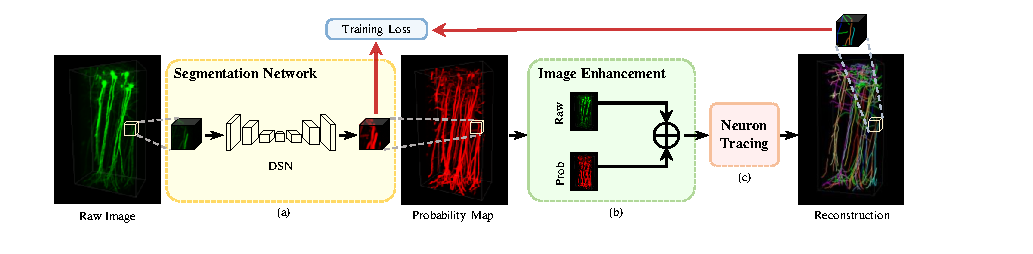
\includegraphics[width=1\textwidth]{./Illustrations/framework2.pdf}
	\caption{Diagram of our progressive learning algorithm for neuron reconstruction in an image block. (a) The segmentation network extracts neuron signals from the raw image. (b) The output probability map is employed to enhance the raw image in order to preserve both global structures and local signal details, which facilitates the neuron tracing module (c) for more complete neuronal population reconstruction. To train the segmentation network, we use the reconstructed neurons as pseudo labels (red arrows), and iteratively refine the network learning and neuron reconstruction with a set of images. The black arrows show the reconstruction pass from an image during testing.}
	\label{fig:framework}
\end{figure*}

Another main bottleneck of existing large-scale neuron reconstruction methods~\cite{Zhou2015, Peng2017, Wang2018} is that they mainly focus on large-scale single neuron reconstruction and the images they processed usually contain only one single neuron. However, a large-scale OM brain image often contains dense neuronal populations in practice.
%
To reconstruct dense neuronal populations from large-scale or even ultra-large-scale noisy images, we introduce UltraNPR, a block-by-block tracing algorithm which utilizes the proposed deep-learning based PLNPR method as the base tracer and \md{designs a tracing strategy with a fusion algorithm for the large-scale neuronal population reconstruction application}.
%In this work, we introduce UltraNPR, an algorithm designed for reconstructing dense neuronal populations from large-scale or even ultra-large-scale images. UltraNPR reconstructs neuronal populations by progressively improving the completeness of neuronal structure block by block.
%
\delete{Firstly, the large-scale raw image is divided into blocks of the same size.
Since somas are where signals from the dendrites are joined and pass on, UltraNPR begins the reconstruction from the blocks that contain somas.
% which can be detected using existing soma detection methods.
For robust reconstruction from low-quality images, our PLNPR method is applied to trace neurons in each block.
Based on the reconstruction results in already-reconstructed blocks, UltraNPR automatically and adaptively searches the next block to trace.
%For each block containing somas, this reconstruction procedure repeats until no new terminal tips could be detected or the next block contains somas.
%Finally, UltraNPR analyzes the reconstruction results in all blocks, and assembles the matched neurites from adjacent blocks to obtain the final complete neuronal population reconstruction. In our implementation, 
Finally, a fusion algorithm is designed to make the fragmented neurites of a neuron from adjacent blocks can be assembled continuously and smoothly.
In this way, UltraNPR is capable of exploring a large-scale image for neuronal population reconstruction.
}


%%%%%%%%%%%%%%%%%%%%%%%%%%%%%%%%%%%%%%%
A preliminary version of this work appears in~\cite{Zhao2019}, where only the robust neuron reconstruction from local image blocks is investigated. In this paper, we tackle with the more challenging large-scale neuronal population reconstruction.
The contributions of this work are summarized as follows:
\begin{enumerate}
\item We propose a general progressive learning framework along with a neuron segmentation network for neuron reconstruction.
%without using manual annotations.
\item We propose a new large-scale neuronal population reconstruction algorithm which is capable of reconstructing dense neuronal populations from terabyte-sized OM brain images.
\item We build a new dataset called ``VISoR-40" which consists of 40 OM image blocks from mouse cortical regions to facilitate neuroscience research. %learning based methods for microscopic explorations.
%which consists of 40 OM images from mouse cortical regions and contains about 400 neuronal trees. Publishing this dataset will strongly support the study of deep neural networks for microscopic explorations.
\item Extensive experiments on our VISoR-40 dataset and the public BigNeuron dataset demonstrate the effectiveness and superiority of our progressive learning algorithm for neuronal population reconstruction and single neuron reconstruction, respectively.
\end{enumerate}

%%%%%%%%%%%%%%%%%%%%%
%Before proceeding into the detailed account of our approach, it is useful to briefly review the related research efforts.
The remainder of this paper is organized as follows. In Section~\ref{sec:related work}, we make a survey of related work. In Section~\ref{sec:method}, we first introduce the PLNPR algorithm, then elaborate the UltraNPR algorithm. We report the experiment results and discussions in Section~\ref{sec:experiments}. Finally, conclusions are drawn in Section~\ref{sec:conclusion}.
